\chapter{Werking cartridge}
\chapterpreamble

\section{Broncode}

In dit hoofdstuk wordt de werking van de \product uitgelegd. Ondanks dat er redelijk wat details besproken worden blijft deze uitleg relatief oppervlakkig daar een gedetailleerde uitleg een veelvoud aan pagina's zou behoeven. De beschrijvingen in dit hoofdstuk moeten vooral als conceptueel beschouwd worden en voor meer details wordt aangeraden om de originele schema's en broncode op de Github pagina te raadplegen.\\
\url{https://github.com/ifilot/p2000t-sdcard/}

%
%
%
\section{Printplaat}

Het ``hart'' van de \product is de printplaat in de \sleuf{2} cartridge. Een schematische afbeelding van deze printplaat en diens componenten staat afgebeeld in \cref{fig:pcb-design}. Voor het schakelschema, zie pagina \pageref{sec:schematic-cartridge2}.

\begin{figure}[h!]
    \centering
    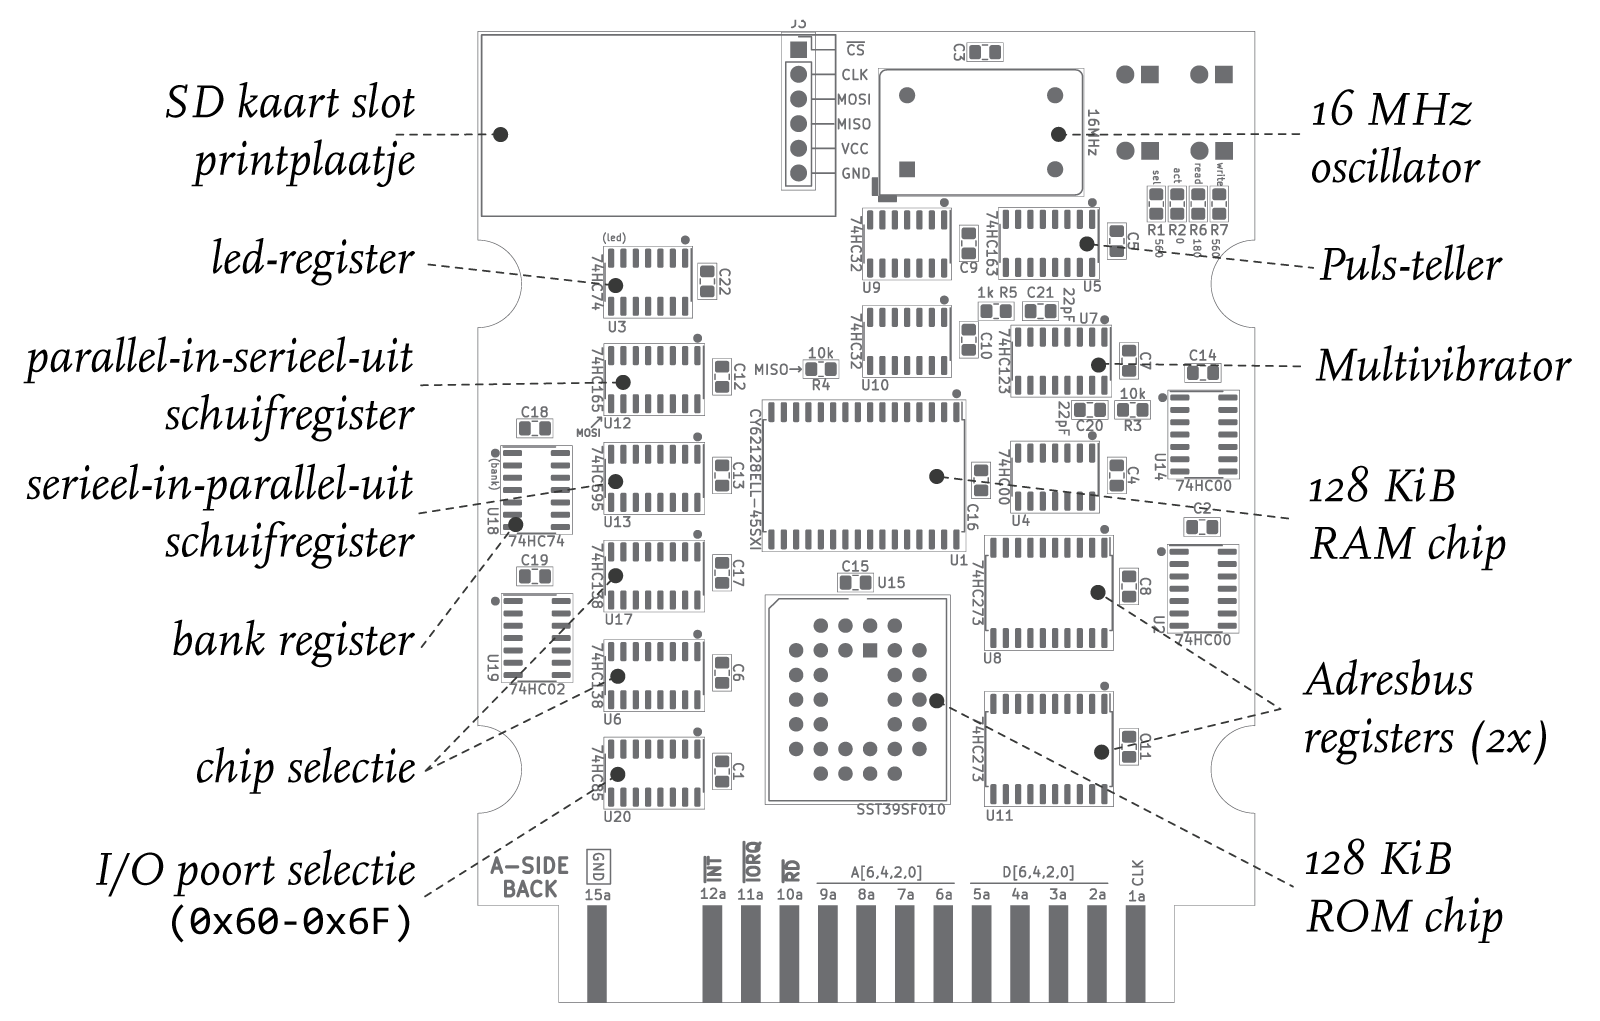
\includegraphics[width=0.99\textwidth]{img/pcb-design}
    \caption{Schematische weergave van de achterzijde van de printplaat en de functionaliteit van de diverse chips.}
    \label{fig:pcb-design}
\end{figure}

De verbinding tussen de \pkb{P2000T} en de SD-kaart is een seriële verbinding conform het SPI protocol. In dit protocol gebeurt de data-overdracht tussen twee apparaten simultaan. Om een byte aan data uit te lezen vanaf de SD-kaart moet er ook eerst een byte ingaan. Dit gebeurt via twee schuifregisters: een parallel-in-serieel-uit (PISU) en een serieel-uit-parallel-in (SUPI) schuifregister.\footnote{In het Engels zijn deze afkortingen PISO en SIPO.} Middels een enkele instructie kan de \pkb{P2000T} een byte aan data wegschrijven in het PISU schuifregister. Vervolgens wordt er gecontroleerd 8 pulsen op 8 MHz aangeslagen om de data vanuit de PISU naar de SD-kaart weg te schrijven. Simultaan worden dan ook 8 bits aan data (1 byte) ontvangen in de andere SIPU register welke wederom middels een enkele operatie door de \pkb{P2000T} uitgelezen kan worden. De pulsen worden gegenereerd door de 16 MHz oscillator welke middels de puls-teller door twee wordt gedeeld om een 8 MHz signaal te geven. De multivibrator zorgt ervoor dat deze pulse-generator niet vroegtijdig voor een tweede keer geactiveerd kan worden. Het grote voordeel van deze opstelling is dat elke machine-instructie van de \pkb{P2000T} optimaal benut kan worden en dat er geen vertraging optreedt bij de parallel-naar-serieel conversie daar deze volledig in hardware verloopt.

De verscheidene componenten op de \sleuf{2} cartridge zijn allen aangesloten op de onderste byte van de adresbus (\pkb{A0-A7}) en de databus (\pkb{D0-D7}). Ze kunnen benaderd worden via I/O poorten \pkb{0x60-0x6F}. Afhankelijk van de specifieke I/O waarde wordt slecht één van de chips geactiveerd.

Naast het SD-kaartje bevat de \sleuf{2} cartridge ook een 128 KiB RAM en 128 KiB ROM chip. Omdat enkel de onderste byte van de adresbus toegankelijk is in \sleuf{2}, moet er gebruikt gemaakt worden van additionele registers om het volledige geheugen op deze chips aan te kunnen spreken. De twee adresbus registers worden gedeeld door de ROM en RAM chip en kunnen tezamen 64 KiB geheugen adresseren. Middels een 2 x 1-bit bank register kan hiermee ofwel de onderste of de bovenste 64 KiB van de 128 KiB benaderd worden. Het bank register wordt niet door de RAM en ROM chips gedeeld; elke chip heeft zijn eigen 1-bit register.

Tenslotte heeft de \sleuf{2} cartridge vier LED-lampjes. De bovenste twee LED-lampjes worden puur hardwarematige aangestuurd. Wanneer de SD-kaart geactiveerd is zal het gele lampje branden. Bij data-overdracht zal het ambergekleurde lampje branden. De onderste twee LEDjes worden softwarematig aangestuurd middels een 2 x 1-bit register.

%
%
%
\section{Geheugenmodel}
\label{sec:memory-model}

De \product gaat uit van verschillende geheugenmodellen van de \pkb{P2000T}. Een overzicht van deze modellen is weergegeven in \cref{fig:memory-models}. De meest basale variant omvat de zogeheten ``kale'' \pkb{P2000T} welke 16 KiB aan geheugen heeft. Dit is de meest beperkende configuratie en bepaalt feitelijk de bovenste limiet van de grootte van de firmware.\footnote{Het doel is namelijk dat de firmware werkt op alle varianten van de \pkb{P2000T} en niet alleen op modellen met een geheugenuitbreiding.} In deze configuratie plaatst de monitor\footnote{De monitor is het stukje code in \pkb{0x0000-0x0FFF} dat o.a. routines bevat voor het toetsenbord, de monitor en het tapedeck. Men kan de monitor zien als de ``BIOS'' van de \pkb{P2000T}.} de top van de stack op \pkb{0x9FFF}. De programmatuur van de \product wordt geplaatst op \pkb{0x7000-0x9CFF} en mag dus maximaal $11520$ bytes beslaan.

\begin{figure}[h!]
    \centering
    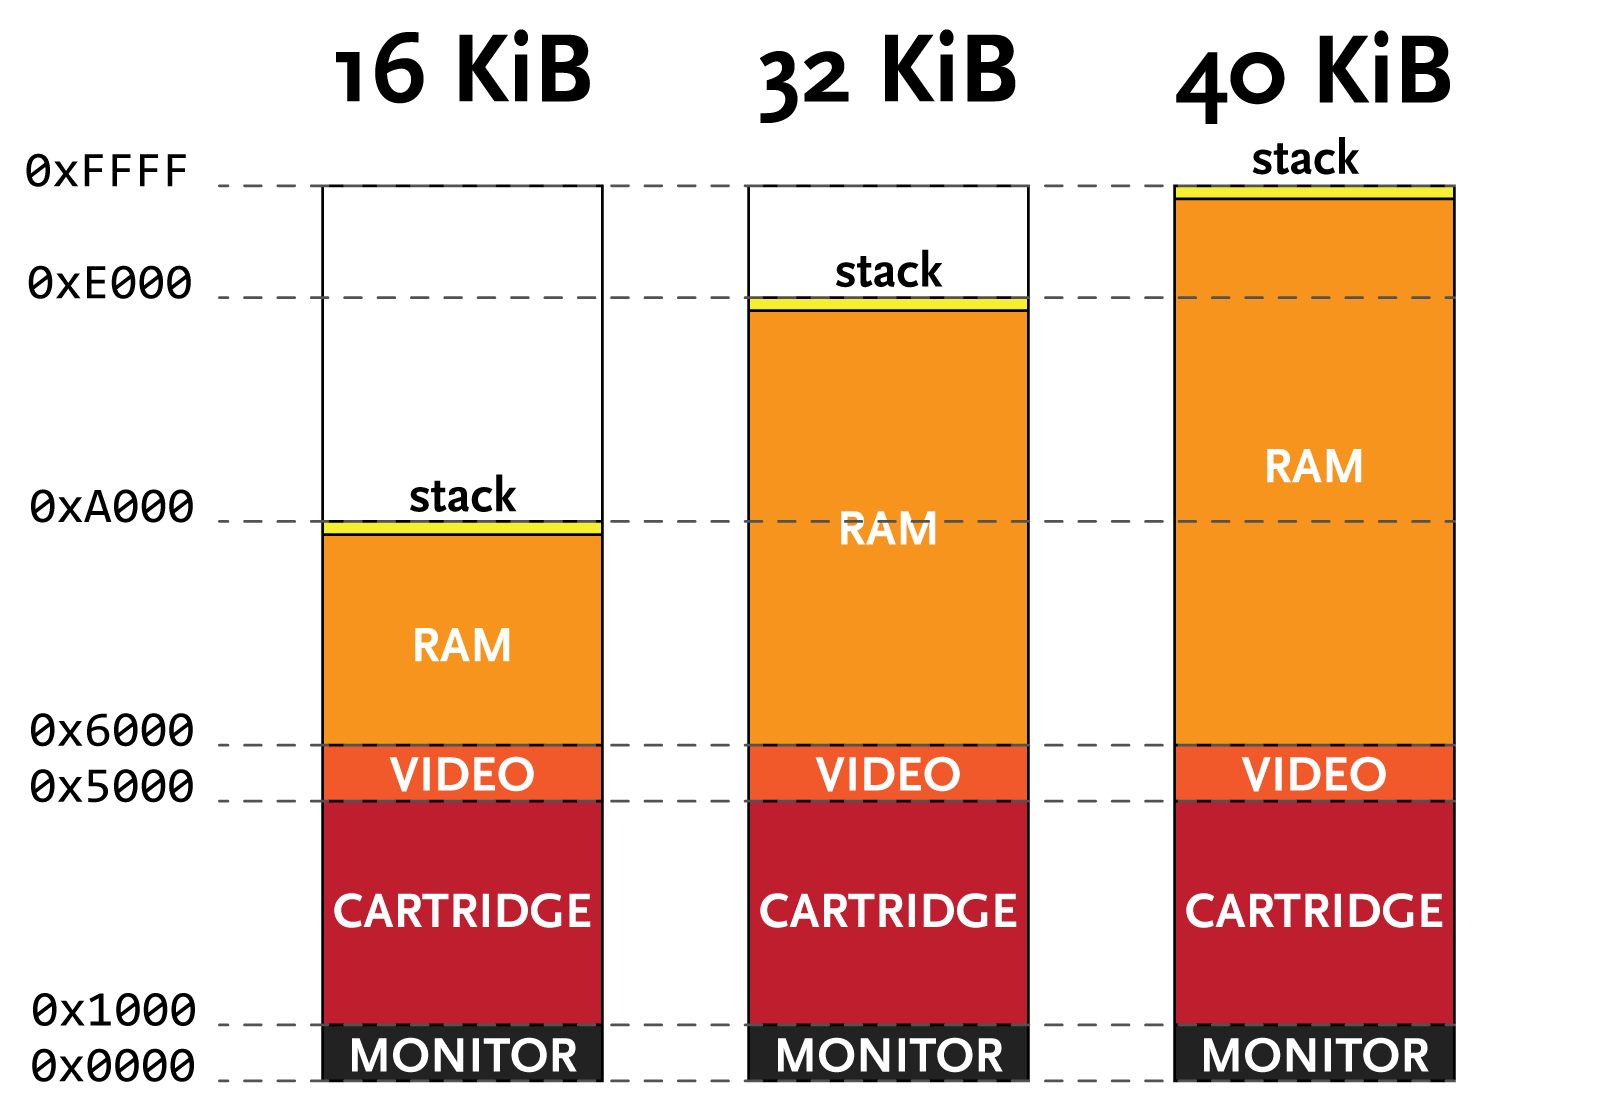
\includegraphics[width=0.99\textwidth]{img/memory_models.png}
    \caption{Geheugenmodellen van de \pkb{P2000T}. De onderste \pkb{0x1000} bytes behoren tot de monitor. Het geheugen van de \sleuf{1} cartridge wordt geplaatst op \pkb{0x1000-0x4FFF}. Hierna volgt het videogeheugen op \pkb{0x5000-0x5FFF}. Al het geheugen hierboven is RAM geheugen. De monitor plaatst de stack altijd aan de top van het beschikbare RAM geheugen. Afgezien van eventuele ``bank switching'' mogelijkheden is het maximale RAM geheugen van een \pkb{P2000T} 40 KiB.}
    \label{fig:memory-models}
\end{figure}

In de iets uitgebreidere scenario heeft de \pkb{P2000T} een 16 KiB geheugenuitbreiding en in totaal dus 32 KiB geheugen. Hierdoor wordt het geheugenbereik \pkb{0xA000-0xDFFF} beschikbaar en plaatst de monitor de top van de stack op \pkb{0xDFFF}. De extra 16 KiB aan geheugen kunnen gebruikt worden om \prg programma's op te starten. Deze stand-alone programma's worden geplaatst op \pkb{0xA000-0xDCFF} en hebben hun eigen stack (van maximaal 512 bytes) waarvan de top geplaatst is op \pkb{0xDEFF}. Deze positie van de stack zorgt ervoor dat de programma's niet kunnen interfereren met de \basic stack.

In het meest uitgebreide scenario is ook het geheugenbereik \pkb{0xE000-0xFFFF} beschikbaar en wordt de top van de \basic stack op \pkb{0xFFFF} geplaatst. Veelal beschikt de \pkb{P2000T} dan ook over ``bank switching'' waarbij het bovenste 8 KiB geheugenblok uitgewisseld kan worden voor een ander blok om zo nog meer geheugen aan te kunnen spreken. \prg programma's die gebruik willen maken van \pkb{0xE000-0xFFFF} en de mogelijkheid tot bank switching moeten zorgdragen dat deze operaties niet interfereren met de \basic stack. Dit kan bijvoorbeeld door de bank met de \basic stack eerst uit te wisselen voor een andere bank.

%
%
%
\section{Opstartprocedures}

%
%
\subsection{CAS bestanden}

Om \cas bestanden in te kunnen laden en af te spelen heeft de \product een \basic omgeving nodig in het geheugenbereik \pkb{0x1000-0x4FFF}. Deze \basic omgeving wordt ingeladen via de \sleuf{1} cartridge, volledig in lijn hoe deze ook normaliter ingeladen wordt. Er zijn echter wel enkele aanpassingen aan deze \basic versie gedaan zodat deze bij het opstarten niet meteen naar de \basic prompt toe gaat, maar juist de \launcher inlaadt van de \sleuf{2} ROM in het interne geheugen en deze opstart. Een diagram van het verloop is weergeven in \cref{fig:loading-cas-file}.

\begin{figure}[h!]
    \centering

    \tikzstyle{block} = [draw, fill=white, rectangle, 
    minimum height=3em, minimum width=6em, rounded corners,
    text width=4.5cm, align=center]

    \tikzset{every picture/.style=thick}
    
    \begin{tikzpicture}[auto, node distance=1.5cm,>=latex']
        \node [draw, circle, fill=primarycol] (start) {\color{white}START};
        \node [block, below of=start] (node0) {\ttfamily\faDownload\;BASIC};
        \node [block, below of=node0] (node1) {\ttfamily\;LAUNCHER\\\faCopy\;ROM $\longmapsto$ eRAM};
        \node [block, below of=node1] (node2) {\ttfamily \faCogs\;LAUNCHER};
        \node [block, below of=node2] (node3) {\faMousePointer\;Gebruiker kiest programma};
        \node [block, below of=node3] (node4) {\ttfamily CAS\\\faCopy\;SD $\longmapsto$ eRAM};
        \node [block, below of=node4] (trash) {\ttfamily \faTrash iRAM};        
        \node [block, below of=trash] (node5) {\ttfamily CAS\\\faCopy\;eRAM $\longmapsto$ iRAM};
        \node [block, below of=node5] (node6) {\ttfamily\faCogs\;CAS};
        \node [draw, circle, fill=primarycol, below of=node6] (stop) {\color{white}STOP};
    
           
        \draw [->] (start) -- (node0);
        \draw [->] (node0) -- (node1);
        \draw [->] (node1) -- (node2);
        \draw [->] (node2) -- (node3);
        \draw [->] (node3) -- (node4);
        \draw [->] (node4) -- (trash);
        \draw [->] (trash) -- (node5);
        \draw [->] (node5) -- (node6);
        \draw [->] (node6) -- (stop);
    
    \end{tikzpicture}
    \caption{Opstartprocedure van \cas bestanden. De betekenis van de symbolen zijn als volgt: \faDownload \; opstarten vanaf cartridge, \faCopy \; kopiëren van data, \faCogs \; uitvoeren van machinecode, \faMousePointer \; gebruikersinvoer, \faTrash - wissen geheugen. iRAM en eRAM staan respectievelijk voor het interne en externe (cartridge) RAM geheugen. ROM staat voor het \sleuf{2} ROM geheugen.}
    \label{fig:loading-cas-file}
\end{figure}

Het opstarten van de \launcher resulteert in het verschijnen van een gebruikersinterface waarmee de gebruiker de SD-kaart kan navigeren en het gewenste programma kan inladen en uitvoeren (\cref{chap:usage}). Bij het uitkiezen van een \cas bestand wordt de programmadata gekopieerd naar het externe RAM geheugen van de cartridge. Hierbij wordt meteen alle metadata (de header informatie) gestript. Uit deze metadata wordt enkel nog de programmagrootte en het plaatsingsadres opgeslagen.

De \launcher wordt nu uit het geheugen gehaald om plaats te maken voor het \cas programma. Het programma wordt, gebruikmakende van de opgeslagen metadata, gekopieerd van het externe RAM naar het interne RAM en uitgevoerd. De gebruiker belandt nu in het gekozen programma en enige restanten van de \launcher zijn niet meer beschikbaar. De gebruiker kan ook niet meer terugkeren naar de \launcher en bevindt zich feitelijk in een \basic omgeving.

%
%
\subsection{PRG bestanden}

Het opstarten van \prg bestanden is redelijk vergelijkbaar met de procedure voor het opstarten van \cas betanden. Er zijn twee essentiële verschillen. Allereerst worden \prg bestanden per definitie altijd geplaatst in het geheugenblok \pkb{0xA000-0xDCFF}. Deze \prg bestanden hebben hun eigen stack welke aangemaakt worden tijdens het opstarten van het programma en weer opgeruimd wordt bij beëindiging van het programma. Tevens wordt de stack pointer bij het beëindigen van het programma weer geplaatst op de positie van de de oude stack waardoor men terugkeert naar de \launcher.

\begin{figure}[h!]
    \centering

    \tikzstyle{block} = [draw, fill=white, rectangle, 
    minimum height=3em, minimum width=6em, rounded corners,
    text width=4.0cm, align=center]

    \tikzset{every picture/.style=thick}
    
    \begin{tikzpicture}[auto, node distance=1.5cm,>=latex']
        \node [draw, circle, fill=primarycol] (start) {\color{white}START};
        \node [block, below of=start] (node0) {\ttfamily\faDownload\;BASIC};
        \node [block, below of=node0] (node1) {\ttfamily\;LAUNCHER\\\faCopy\;ROM $\longmapsto$ eRAM};
        \node [block, below of=node1] (node2) {\ttfamily \faCogs\;LAUNCHER};
        \node [block, below of=node2] (node3) {\faMousePointer\;Gebruiker kiest programma};
        \node [block, below of=node3] (trash1) {\ttfamily \faTrash iRAM};
        \node [block, below of=trash1] (node4) {\ttfamily PRG\\\faCopy\;SD $\longmapsto$ iRAM\\\pkb{0xA000-0xDCFF}};
        \node [block, below of=node4] (trash2) {\ttfamily \faTrash iRAM};
        \coordinate [right=1cm of trash2] (coord);
           
        \draw [->] (start) -- (node0);
        \draw [->] (node0) -- (node1);
        \draw [->] (node1) -- (node2);
        \draw [->] (node2) -- (node3);
        \draw [->] (node3) -- (trash1);
        \draw [->] (trash1) -- (node4);
        \draw [->] (node4) -- (trash2);
        \draw [-] (trash2) -- (coord);
        \draw [->] (coord) |- (node2);
    
    \end{tikzpicture}
    \caption{Opstartprocedure van \prg bestanden. De betekenis van de symbolen zijn als volgt: \faDownload - opstarten vanaf cartridge, \faCopy \;kopiëren van data, \faCogs \; uitvoeren van machinecode, \faMousePointer \; gebruikersinvoer, \faTrash \; wissen geheugen. iRAM en eRAM staan respectievelijk voor het interne en externe (cartridge) RAM geheugen. ROM staat voor het \sleuf{2} ROM geheugen.}
    \label{fig:loading-cas-file}
\end{figure}

%
%
%
\section{SD-kaart}

De firmware probeert verbinding te maken met de SD-kaart en de eerste partitie op die kaart te benaderen. De \product kan enkel verbinding maken met SD-kaarten van het type SDHC welke geformatteerd moeten zijn met een FAT32 bestandssysteem. Voor het communiceren met de SD-kaart wordt gebruikt gemaakt van een protocol dat uitgaat van 6-byte instructies, welke beschreven staan in het document ``SD Card Physical Specification''.\footnote{Men kan dit document het beste vinden door deze term in te voeren in een zoekmachine.}

Om de SD-kaart in te lezen worden eerst 96 pulsen gestuurd om deze te laten ontwaken. Middels \cmd{0} wordt de kaart gereset hetgeen gevolgd wordt door \cmd{8}. Vervolgens wordt herhaaldelijk \pkb{CMD55 + ACMD41} gestuurd totdat de SD-kaart respondeert met de waarde \pkb{0x00}. Tenslotte wordt \cmd{58} gestuurd waarna de SD-kaart klaar is om lees- of schrijf-instructies te ontvangen middels \cmd{17} en \cmd{24}. Zie \cref{fig:sd-card-protocol} voor een diagrammatische weergave van het protocol.

\begin{figure}[h!]
    \centering
    \tikzstyle{block} = [draw, fill=white, rectangle, 
    minimum height=3em, minimum width=6em, rounded corners]
    
    \tikzset{every picture/.style=thick}

    \begin{tikzpicture}[auto, node distance=1.5cm,>=latex']
        \node [draw, circle, fill=primarycol] (start) {\color{white}START};
        \node [block, below of=start] (cmd0) {\ttfamily CMD0};
        \node [block, below of=cmd0] (cmd8) {\ttfamily CMD8};
        \node [block, below of=cmd8] (acmd41) {\ttfamily CMD55 + ACMD41};
        \node [draw, diamond, below=0.5cm of acmd41] (lees) {Lees \ttfamily 0xFF\normalfont ?};
        \node [block, below= 0.5cm of lees] (cmd58) {\ttfamily CMD58};
        \node [draw, circle, below=0.5cm of cmd58, fill=primarycol] (stop) {\color{white}ACTIEF};
        \node [block, right=1.5cm of stop] (cmd17) {\ttfamily CMD17};
        \node [block, left=1.5cm of stop] (cmd24) {\ttfamily CMD24};
    
        \coordinate [right=0cm and 2cm of lees] (path) {};
        \coordinate [above=0.3cm of cmd17] (cmd17t) {};
        \coordinate [above=0.3cm of cmd24] (cmd24t) {};
    
        \draw [->] (start) -- (cmd0);
        \draw [->] (cmd0) -- (cmd8);
        \draw [->] (cmd8) -- (acmd41);
        \draw [->] (acmd41) -- (lees);
        \draw [->] (lees) -- node {ja} (cmd58);
        \draw [-] (lees) -- (path);
        \draw [->] (path) |- node [near end] {nee} (acmd41);
        \draw [->] (cmd58) -- (stop);
        \draw [->] (stop) -- (cmd17);
        \draw [->] (stop) -- (cmd24);
        \draw [->] (cmd17) -- (cmd17t) -| (stop.north east);
        \draw [->] (cmd24) -- (cmd24t) -| (stop.north west);
        
    
    \end{tikzpicture}
    \caption{Diagram van het communicatieprotocol met de SD-kaart. Middels een serie van commando's wordt de SD-kaart in een staat geprepareerd waardoor middels \cmd{17} en \cmd{24} een sector (512 bytes) uitgelezen, respectievelijk weggeschreven kan worden.}
    \label{fig:sd-card-protocol}
\end{figure}

In onderstaande lijst staat welk commando welke operaties uitvoeren op de SD-kaart.

\begin{itemize}
    \item \cmd{0}: Reset de SD-kaart.
    \item \cmd{8}: Controleert op welke spanningen de SD-kaart kan opereren.
    \item \cmd{41}: Activeert het initialisatie-proces van de SD-kaart. Omdat dit even duurt, wordt herhaaldelijk getoetst of de SD-kaart gereed is.
    \item \cmd{58}: Lees het OCR (operation condition register) uit.
    \item \cmd{17}: Lees een sector.
    \item \cmd{24}: Schrijf een sector.
\end{itemize}

%
%
%
\section{FAT32}

De communicatie met de SD-kaart betreft enkel ruwe data-overdracht en is onafhankelijk van het bestandssysteem dat op de SD-kaart staat. Om bestanden te kunnen vinden moet de data geïnterpreteerd worden. De \product gaat ervan uit dat de SD-kaart geformatteerd is met een FAT32 bestandssysteem welke relatief makkelijk te gebruiken is. Elke FAT32 partitie, zie \cref{fig:fat32-partition} bestaat uit een sector met partitie-informatie (VOLUME ID), gevolgd door enkele gereserveerde sectoren, daarna twee FATs (file allocation tables) en tenslotte een hele reeks clusters.

\begin{figure}[h!]
    \centering
    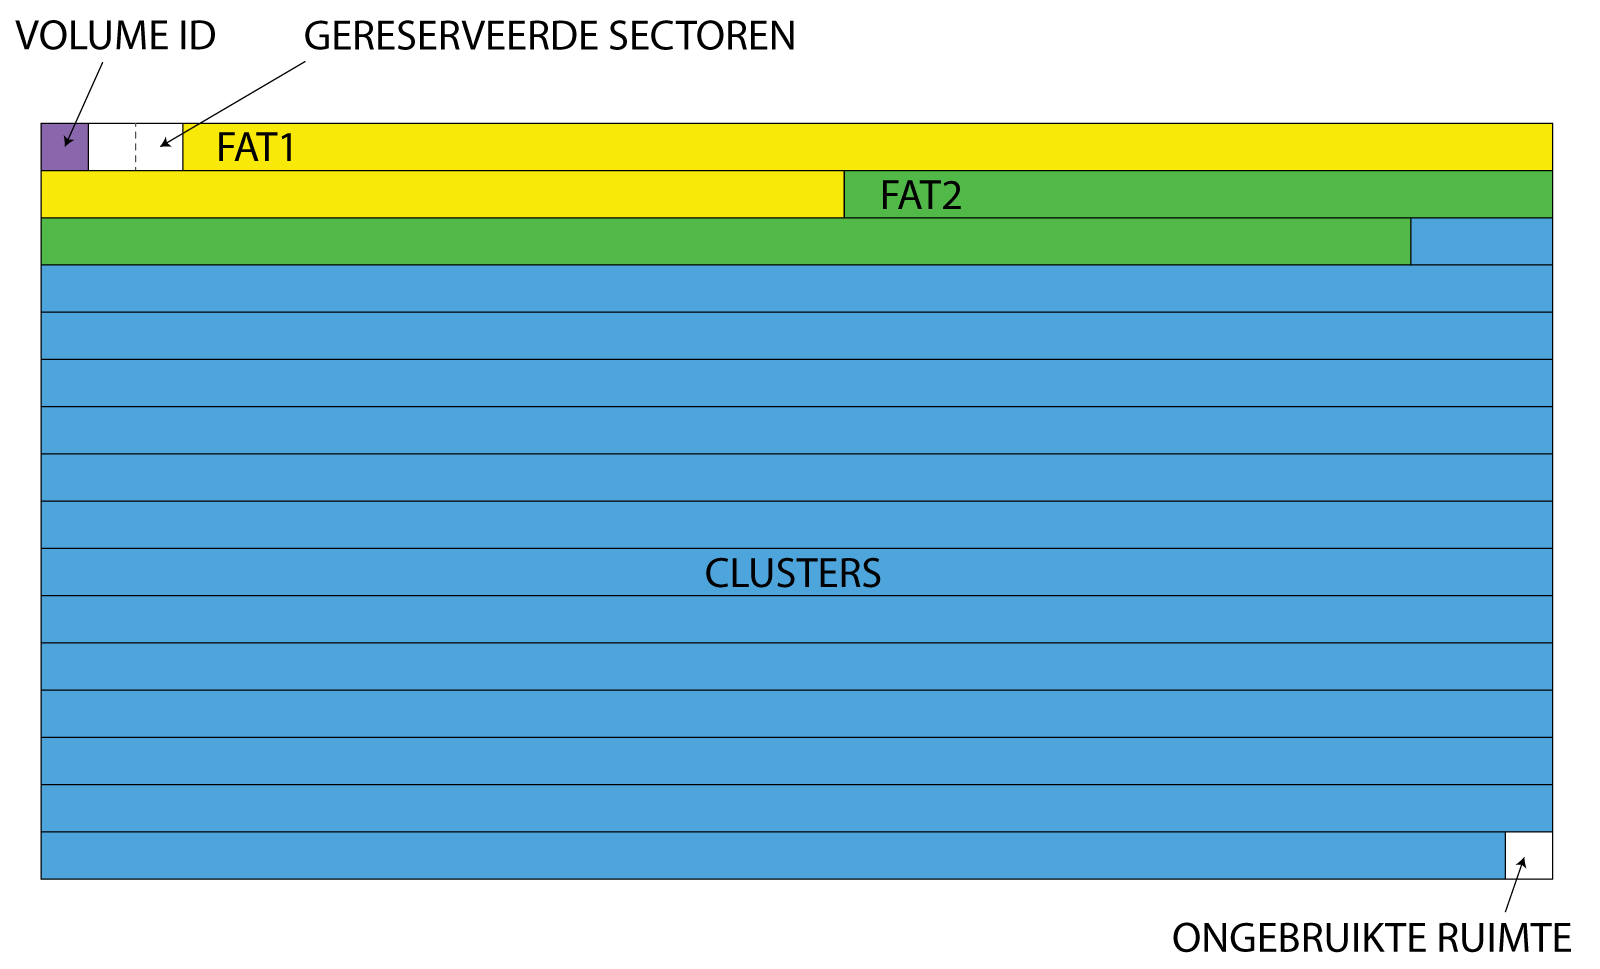
\includegraphics[width=0.70\textwidth]{img/fat32-partitie.png}
    \caption{Partitie-indeling van een FAT32 bestandssysteem.}
    \label{fig:fat32-partition}
\end{figure}

Bij het inlezen van een SD-kaart wordt eerst de boot-sector gelezen (\cref{fig:boot-sector}). Dat is de eerste sector op het SD-kaartje en deze geeft per partitie aan waar dat de partitie zich bevindt. Deze sector heeft aan het einde de 16-bit signatuur \pkb{0x55AA} welke gebruikt kan worden ter controle of deze sector correct is uitgelezen.

\begin{figure}[h!]
    \begin{subfigure}[t]{0.3\textwidth}
        \centering
        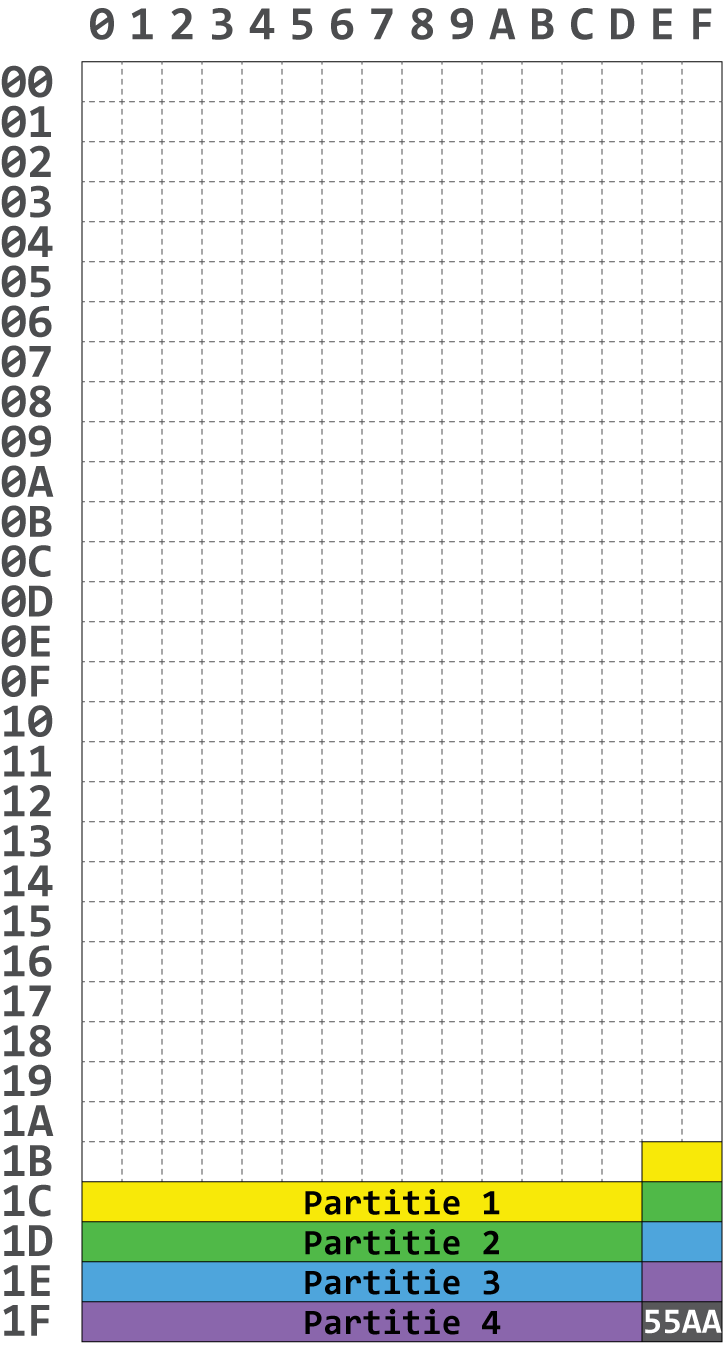
\includegraphics[width=0.95\textwidth]{img/boot-sector.png}
        \caption{Boot-sector}
        \label{fig:boot-sector}
    \end{subfigure}%
    ~ 
    \begin{subfigure}[t]{0.7\textwidth}
        \centering
        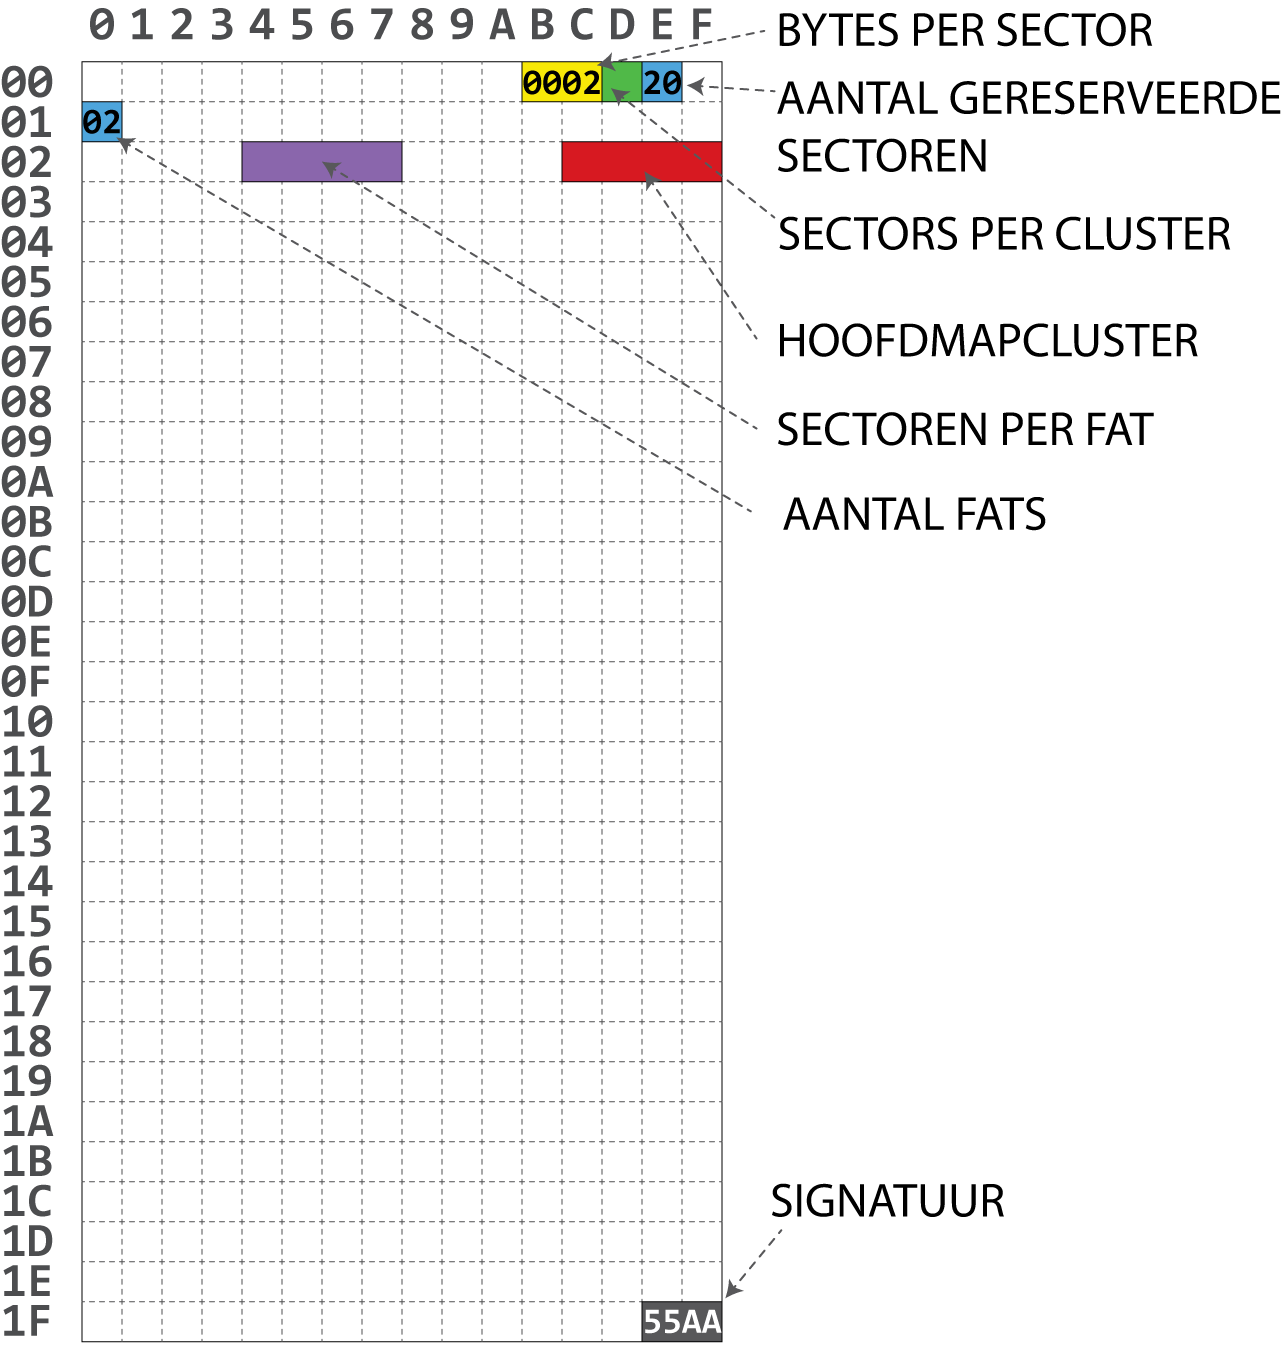
\includegraphics[width=0.95\textwidth]{img/volume-id.png}
        \caption{Eerste sector van een partitie}
        \label{fig:volume-id}
    \end{subfigure}
    \caption{(a) Boot-sector van de SD-kaart en (b) eerste sector van een partitie met aanduiding van de relevante partitiegevens.}
\end{figure}

Op basis van de boot-sector kan de eerste sector van een partitie gevonden worden (\cref{fig:volume-id}). Op deze sector staat een reeks aan belangrijke gegevens om de partitie uit te kunnen lezen. Sommige van deze gegevens staan in principe altijd vast voor FAT32 bestandssystemen, zoals het aantal bytes per sector (512 bytes), het aantal gereserveerde sectoren (20) en het aantal FATs (2). Andere zaken hangen af van de formatteerinstellingen. Zo kan tijdens het formatteren met een FAT32 bestandssysteem de clustergrootte gekozen worden, welke het aantal sectoren per cluster en het aantal sectoren per FAT bepaald. Op basis van het aantal sectoren per FAT en het aantal sectoren per cluster kan de totale capaciteit van de partitie uitgerekend worden. Ook staat in de eerste sector van de partitie het clusteradres van de hoofdmap. Dit adres bepaalt waar we moeten beginnen met lezen wanneer we het bestandssysteem willen navigeren.

\begin{figure}[h!]
    \begin{subfigure}[t]{0.6\textwidth}
        \centering
        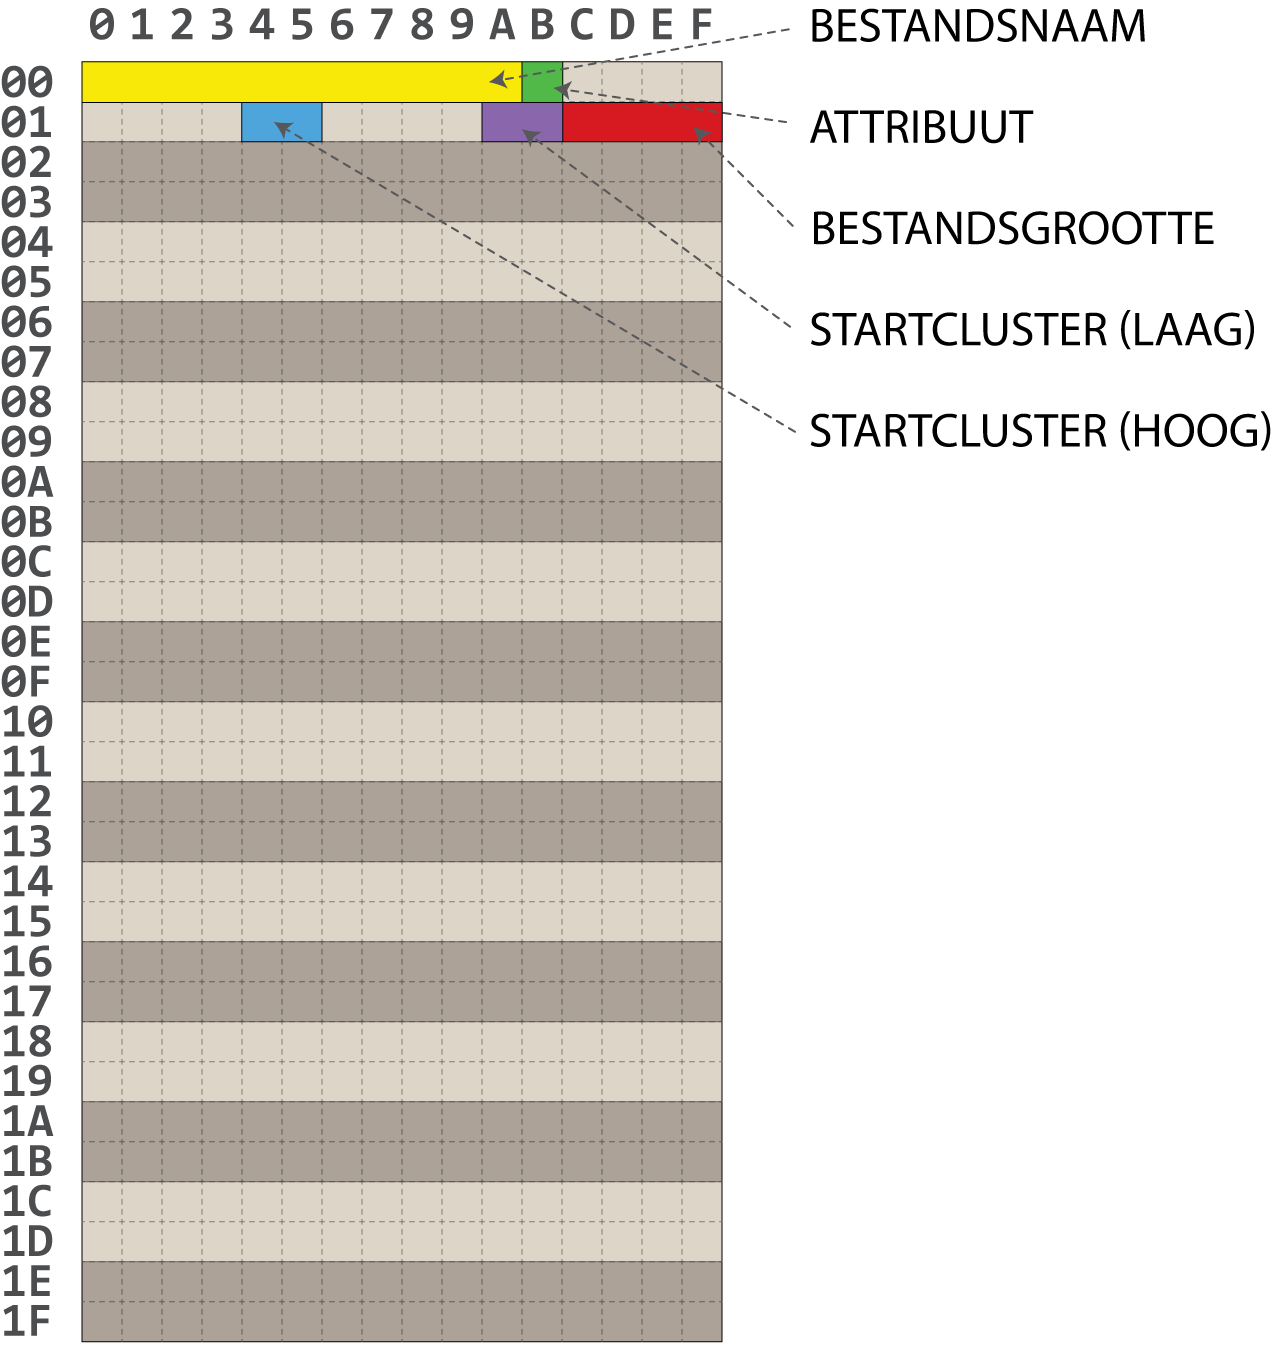
\includegraphics[width=0.95\textwidth]{img/folder-cluster.png}
        \caption{Folder sector.}
        \label{fig:folder-cluster}
    \end{subfigure}%
    ~ 
    \begin{subfigure}[t]{0.4\textwidth}
        \centering
        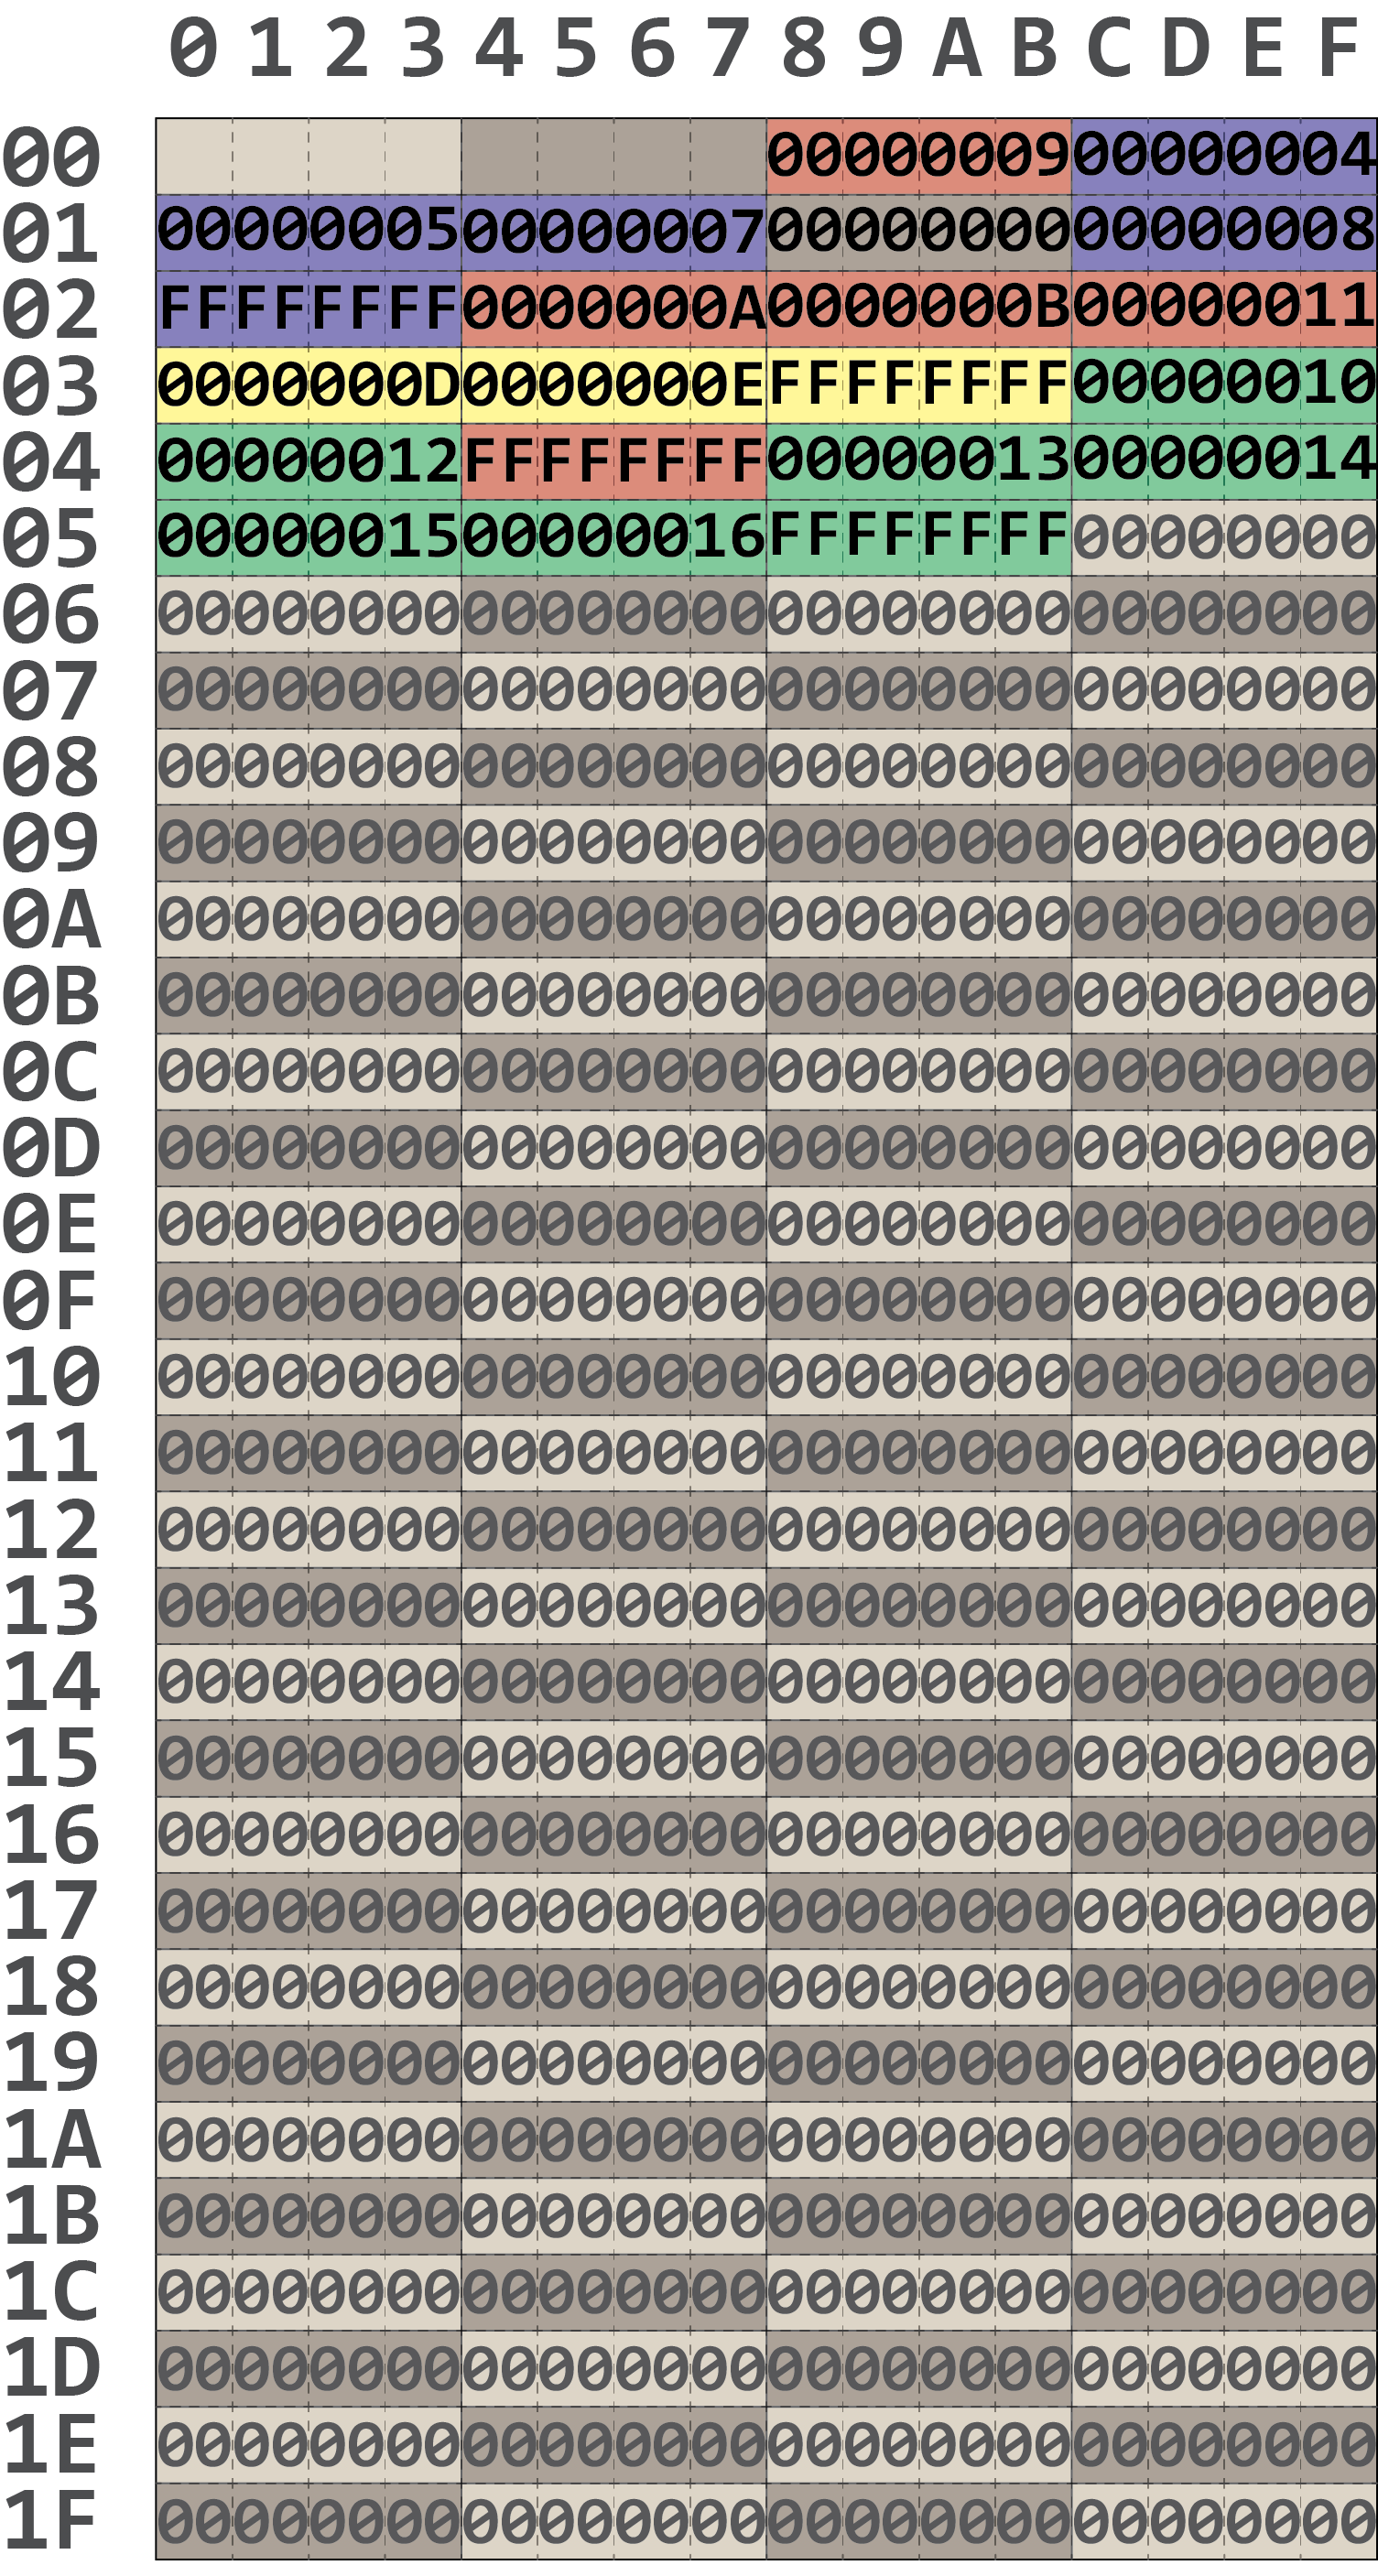
\includegraphics[width=0.95\textwidth]{img/fat32-voorbeeld.png}
        \caption{FAT sector.}
        \label{fig:fat-example}
    \end{subfigure}
    \caption{(a) Sector van een folder en (b) een sector van een FAT.}
\end{figure}

In \cref{fig:folder-cluster} staat een voorbeeld gegeven van een cluster welke behoort tot een folder. Dit cluster is opgedeeld in blokjes van 32 bytes waarbij elke blokje een omschrijving (metadata) bevat van een bestand of een subfolder. Of het stukje data een bestand of een folder beschrijft valt te bepalen aan de attribuutbyte. Het stukje metadata bevat ook een 32-bit clusteradres opgedeeld in een hoog 16-bit en een laag 16-bit fragment van dit adres. Tenslotte wordt ook de grootte van het bestand opgeslagen zodat bepaald kan worden hoeveel sectoren uitgelezen zouden moeten worden. 

Het clusteradres vormt echter enkel het eerste adres van een bestand of subfolder en een bestand of folder kan groter zijn dan een enkel cluster. In dat geval moet men weten welke clusters volgen na het eerste cluster. Dit is de functie van de FAT. De FAT geeft per cluster aan of er een vervolgcluster is. Als er geen vervolgcluster is, dan staat er in de FAT de waarde \pkb{0xFFFFFFFF}. Als er wel een vervolgcluster is, dan wordt het nummer van dit vervolgcluster genoemd. Vervolgens kan dit vervolgcluster ook weer een volgend cluster hebben en zo kunnen we dit proces blijven herhalen totdat er het adres \pkb{0xFFFFFFFF} gevonden wordt voor een cluster. Zie ter illustratie \cref{fig:fat-example}. Deze FAT geeft bijvoorbeeld aan (met de rode blokjes) dat er een bestand of cluster zich bevindt in de clusters \pkb{0x00000003}, \pkb{0x00000009}, \pkb{0x0000000A}, \pkb{0x0000000B} en tenslotte \pkb{0000011}; 5 clusters dus in totaal. Een ander voorbeeld betreft een bestand of folder aangegeven met de blauwe clusters. Dit bestand of folder omvat de clusters \pkb{0x00000003}, \pkb{0x00000004}, \pkb{0x00000005}, \pkb{0x00000007} en tenslotte \pkb{0x00000008}. Clusters met adres \pkb{0x00000000} zijn lege clusters welke nog opgevuld kunnen worden met data.

%
%
%
\section{Bestandsformaten}

\subsection{CAS bestanden}
\label{sec:cas-files}

\cas bestanden zijn een bestandsformaat bedacht in 1996\footnote{\url{https://www.komkon.org/~dekogel/m2000.html}} door Marcel de Kogel om programma's van \pkb{P2000T} cassettes op te slaan op een moderne(re) computer. Deze bestanden bestanden uit \textbf{blokken} van 1280 bytes (\pkb{0x500}) bytes. Elk \textbf{blok} van \pkb{0x500} bytes is weer opgedeeld in een header van \pkb{0x100} bytes en een data gedeelte van \pkb{0x400} bytes. Deze header is een kopie van het geheugen \pkb{0x6000 - 0x6100} tijdens het wegschrijven van de cartridge. Van dit stukje geheugen blijkt (achteraf) alleen het stukje \pkb{0x6040 - 0x605F} relevant voor de beschrijving van het \cas bestand. In \cref{tab:cassette-metadata} staat een overzicht van de informatie die in dit geheugenblok opgenomen is.

\begin{table}
\caption{Omschrijving van de relevante data voor een cartridge in geheugenblok \pkb{0x6040 - 0x605F}.}
\label{tab:cassette-metadata}
\centering
\begin{tabular}{|r|l|}
\hline
Adres & Omschrijving \\
\hline
\pkb{0x6030-0x6031} & Transfer adres \\ \hline
\pkb{0x6032-0x6033} & Bestandsgrootte \\ \hline
\pkb{0x6034-0x6035} & Record grootte \\ \hline
\pkb{0x6036-0x603D} & Label (1/2) \\ \hline
\pkb{0x603E-0x6040} & Extensie \\ \hline
\pkb{0x6041-0x6042} & Type \\ \hline
\pkb{0x6043-0x6044} & Startadres \\ \hline
\pkb{0x6045-0x6046} & Load \\ \hline
\pkb{0x6047-0x604E} & Label (2/2) \\ \hline
\pkb{0x604F} & Aantal resterende blokken bij inlezen \\
\hline
\end{tabular}
\end{table}

%
%
\subsection{PRG bestanden}
\label{sec:prg-files}

\prg bestanden zijn speciale machinecode bestanden gemaakt voor de \product. Deze bestanden hebben een 16-byte header, worden op een vaste positie in het geheugen geplaatst en uitgevoerd met een nieuwe stack. De bestanden worden geplaatst op \pkb{0xA000-0xDCFF} en mogen maximaal \pkb{0x3D00} bytes lang zijn.\footnote{Ongeveer 15.25 KiB, net iets minder dan de grootte van een cartridge ROM, welke 16 KiB is.} De stack voor deze bestanden begint op \pkb{0xDEFF} en loopt afwaarts naar \pkb{0xDD00}, hetgeen een stackgrootte van 512 bytes geeft. Voor het draaien van \prg bestanden heeft men tenminste een 16 KiB geheugenuitbreiding nodig. Indien er enkel een 16 KiB geheugenuitbreiding aanwezig is (en niet meer) op de \pkb{P2000T}, dan zal de stack voor \basic en het menu zich bevinden in \pkb{0xDF00-0xDFFF} waardoor dit stukje geheugen onaangetast moet blijven.

De header van de \prg bestanden is vergelijkbaar met de header voor \sleuf{1} cartridges. Het eerste karakter dient altijd een \pkb{0x50} te zijn, corresponderend met de ASCII waarde voor de hoofdletter \pkb{P}. Hierna volgen 2 x 16-bit waarden\footnote{In little-endian notatie, zie \cref{sec:endianness} op Pagina \pageref{sec:endianness}.}, corresponderend met het aantal bytes van het programma gevolgd door de CRC-16 checksum.\footnote{Zie \cref{sec:crc16-checksum} op Pagina \pageref{sec:crc16-checksum} voor meer informatie over CRC-16 checksums.} Deze CRC-16 checksum begint vanaf positie \pkb{0x10}, dus na de 16-byte header. Tenslotte resteren 11 karakters die de gebruiker vrij mag invullen, maar waarvan wordt aangeraden om een 8+3 bestandsnaam te gebruiken.

In tegenstelling tot \cas bestanden keren \prg bestanden wel terug naar het menu wanneer deze afgesloten worden. Om die reden is het programma opgeslagen in de \prg bestanden zelf verantwoordelijk voor het aanmaken en opruimen van de stack en het herpositioneren van de stackpointer \pkb{SP}. Middels de \pkb{Z88dk} toolchain is het echter vrij eenvoudig om dit op te stellen.